\section{Evaluation}

We evaluated the timing compartments architecture using the gem5 architectural 
simulator~\cite{gem5} integrated with the DRAMSim2~\cite{DRAMSim2} memory 
simulator. Our experiments use multiprogram workloads comprised of SPEC2006 
benchmarks compiled for the ARM ISA. 

Table~\ref{tab:config} shows our system configuration.
The cores use the gem5 ``O3`` out-of-order core model which runs at 2GHz.  Each 
core has private 32KB L1 instruction and data caches, and private 256KB L2 
cache. The cores share a 4MB L3 cache. We derived cache configuration 
parameters from the Intel Xeon E3-1220L, which is a two core architecture used 
by Amazon EC2. In DRAMSim2, we simulate a 667MHz 2GB DDR3 memory. The 
interconnects in the simulator runs at 1GHz. Unless specified otherwise, each 
experiment is fastforwarded for 1 billion instructions, and run for 100 million 
instructions. 

%We will first describe our security evaluation and then show
%the performance evaluation.

\begin{table}
    \caption{Simulator configuration parameters.}
    \centering
\begin{small}
    \begin{tabular}{|l|l|l|r|}
        \hline
        \multicolumn{3}{|l|}{gem5 core model} & ``O3''        \\\hline
        \multicolumn{3}{|l|}{CPU Clock}    & 2GHz             \\\hline
        \hline
        \multicolumn{2}{|l|}{Memory}             & 2GB    & 667MHz  \\\hline
        \hline
        \multicolumn{3}{|l|}{Network Clock}      & 1GHz \\\hline
        \hline
        L1d / L1i  & 32kB   & 2-way  & 2 cycles\\\hline
        L2         & 256kB  & 8-way  & 7 cycles \\\hline
        L3         & 4MB    & 16-way & 17 cycles  \\\hline
    \end{tabular}
    \end{small}
    \label{tab:config}
\end{table}

\subsection{Security}

At a high level, the general approach that we use such as static partitioning,
duplication, and TDM should remove timing interference. We experimentally
tested the security in order to check if we miss any sources of timing interference.
%To experimentally evaluate the security of our architecture, 
The experiments simulate a two-core 
system with two timing compartments, TC0 and
TC1, running concurrently. 
%The protection policy is configured to disallow any 
%timing channels between the two compartments. 
If the timing isolation is complete, then the execution time of a program on 
TC0 should be independent of the workload on TC1.
%If the number of cycles required 
%to execute a certain number of instructions for a particular benchmark running
%on TC0 depends on which benchmark is running on TC1, it indicates timing 
%interference still exist. In a secure system, the execution time
%of TC0 would be unaffected by TC1. 
Using this reasoning, we checked the
security of our design by running, a fixed benchmark
on TC0 wihle varying the benchmark on TC1 and compared the execution times. 
As expected, 
%these tests showed interference in the baseline without protection.
%On the other hand,
we observed no interference with timing compartments enabled.

\subsection{Time Slice Coordination}
\label{sec:eval_coord}

To explore a large design space of coordinating the time slices for the TDM 
protection schemes, we built a custom simulator that only models the memory
hierarchy for an L2 cache miss.
Given the turn lengths and offsets of each device, the L2 miss latency can
be determined based on the cycle in which an L2 miss happens.
Because a schedule repeats after the least common multiple of each turn length in 
the schedule multiplied by the number of timing compartments, each possible 
latency for a schedule can be enumerated. The simulator calculates
the expected L2 miss latency assuming that the timing of L2 misses shows a
uniform random distribution.

Using this simulator, we exhaustively tested the L2 miss latency for an
L3 hit under all possible turn lengths within a limit and all possible
offsets. The experiments confirmed that 
the intuitive schedule described in 
Section~\ref{sec:coordination} achieves the lowest expected L2 miss latency
assuming a hit in the L3 cache.
Fixing the turn lengths to the optimal values and adjusting only the offsets,
the worst case latency is 19.6\% higher than the one with the optimal schedule, showing
the importance of the coordination.
%that coordinating the hit path is important.

The design space for schedules involving all resources from the L2 cache to
the main memory is far too large to search exhaustively.
Instead we used the simulated annealing to search the design space.
%We found that changing a 
%turn length or offset slightly can drastically affect the performance, so the 
%search space has many relative minima. We used our own simulated annealing 
%optimizer to avoid getting stuck at relative minima and increase our chances of 
%finding a global minimum.
First, we used the optimizer to study the L2 miss latency when the access misses
in the L3 as well.
After initializing the optimizer with the L3 miss schedule summarized in 
Figure~\ref{fig:miss_schedules}, the optimizer did not find a better schedule 
after 20,000 iterations. Fixing the turn lengths to be the same as the best 
schedule and sweeping only the space of offsets,
the worst-case schedule resulted in the memory latency that is 2.38X
higher than the best schedule.

We used the same optimizer to study the best schedule to minimize the average
L2 miss latency under the assumption that the L3 cache hit-rate is 90\%.
This case did not have any intuitive solution because the solution needs to 
balance the two schedules that provide low latencies for L3 hits and misses.
%Optimizing for the L2 miss rate overall is a harder problem since it requires a 
%balance bewtween the best L3 miss case and L3 hit case parameters. 
The schedule 
produced by the optimizer was not one that made any intuitive sense.  However, 
the optimal schedule was 8.67X better than the worst schedule that used the 
same turn lengths as the best schedule (and changed only the offsets).

The results for schedule selection study are summarized in Table 
\ref{tab:coord_results}. Overall, scheduling interdependent time multiplexed 
devices is a challenging problem, but the gap between the worst and optimal 
cases show that it is important.

\begin{table}
    \caption{Scheduling Selection Study Results.}
    \begin{small}
    \centering
    \begin{tabular}{|l|l|l|l|}
        \hline
        \multicolumn{1}{|l|}{Optimized Quantity} & Search & Min & Max \\\hline
        \multicolumn{1}{|l|}{L3 Hit Latency} & Exhaustive & 25.5 & 30.5 
        \\\hline
        \multicolumn{1}{|l|}{L3 Miss Latency} & Simulated Annealing& 139.5 & 
        334.5 \\\hline
        \multicolumn{1}{|l|}{L2 Miss Latency} & Simulated Annealing& 38.6 & 
        344.5 \\\hline
    \end{tabular}
    \end{small}
    \label{tab:coord_results}
\end{table}

\subsection{Performance Overhead}

The timing compartment architecture extends the insecure baseline with
static partitioning and time multiplexing to secure the shared hardware 
resources. These changes lead to underutilization, and thus, a performance
overhead. To evaluate the performance overhead, we ran multiprogram workloads 
comprised of pairs of SPEC2006 benchmarks, and measured the execution time of
the benchmark in TC0.
%We configured the security policy to disallow communication among all timing 
%compartments, and measured the execution time of the benchmark
%in TC0. 
Since the timing channel protection mechanisms primarily affect the 
memory hierarchy, the performance overhead heavily depends on the memory intensity 
of the benchmarks.
The memory intensity of each benchmark, in terms of L2 misses per thousand 
instructions, is shown in
Figure~\ref{fig:memstudy}. Of the SPEC2006 benchmarks, mcf has the most L2 misses,
while astar has almost none after fast-forwarding for 1B instructions.

For the baseline architecture, we calculate the average execution time of the 
benchmark on Core 0 by averaging among runs with different benchmarks on Core 
1.  In the baseline, the execution time of the benchmark in Core 0 is impacted by the benchmark 
in Core 1 due to interference in shared resources. 
In the timing compartments architecture, the execution time of TC0 
(on Core 0) is independent of workloads running in other timing compartments.

Figure~\ref{fig:two_tc_overhead} shows the performance overhead when running 
two TCs. Libquantum and mcf incur the highest overhead at 22\% and 10\% 
respectively. However, each other benchmark has an overhead lower than 5\%, and 
the arithmetic mean of the overheads is only 4.3\%
The results show that the overhead of strong timing isolation can be reasonable
for a small number (2) of timing compartments because it only affects infrequent
L2 misses.

\begin{figure}
    \begin{center}
        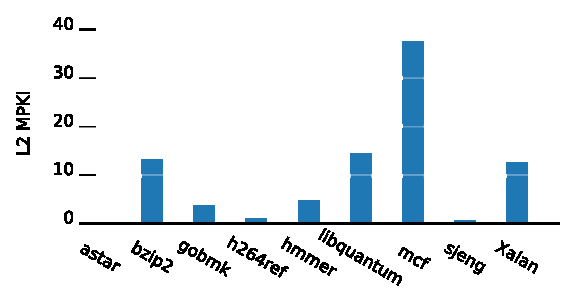
\includegraphics[width=3.4in]{figs/MPKI.eps}
        \caption{Memory intensity of SPEC2006 benchmarks.}
        \label{fig:memstudy}
    \end{center}
\end{figure}

\begin{figure}
   \begin{center}
       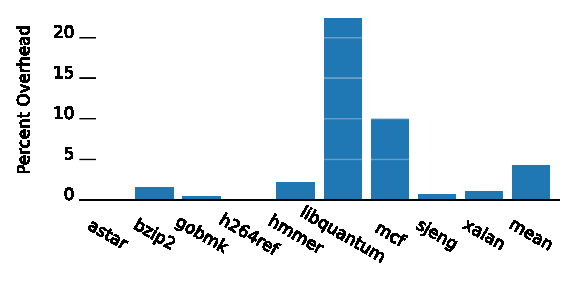
\includegraphics[width=3.4in]{figs/two_tcs.eps}
       \caption{Percent overhead of two timing compartments.}
       \label{fig:two_tc_overhead}
   \end{center}
\end{figure}

% Figure~\ref{fig:performance} shows the performance overhead of full system 
% protection as well as the overhead incurred by the changes to the memory 
% controller (mc), the cache (waypart), the L3 to memory bus (membus), and the 
% L2 to L3 bus (L2L3) individually compared to the insecure baseline. The
% overheads for libquantum and mcf, which are particularly memory intensive, 
% are highest at 69\% and 18\% respectively. However, the arithmetic mean of 
% the total overhead is quite low at roughly 9\%. Memory controller protection 
% incurs by far the most overhead suggesting the impact on memory bandwidth is 
% more significant than bus or cache underutilization. Overall, the results 
% show that the timing compartments are viable for applications that require 
% high assurance for software isolation.

% \begin{figure}
%     \begin{center}
%         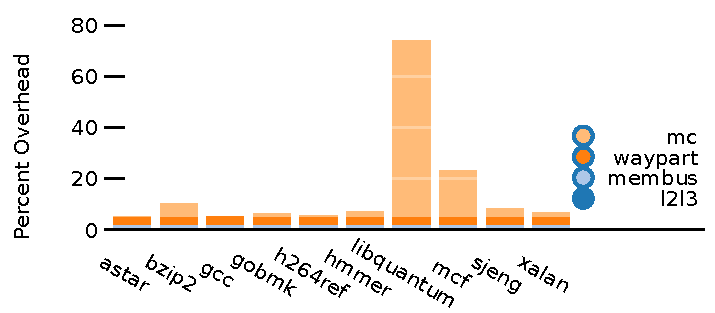
\includegraphics[width=3.4in]{figs/breakdown.pdf}
%         \caption{Performance overhead for 2 TCs.}
%         \label{fig:performance}
%     \end{center}
% \end{figure}

The performance overhead is likely to increase as the number of timing 
compartment scales up. To study the impact of the number of timing 
compartments, we evaluated the performance overhead with two, three, and four 
timing compartments on a 4-core  processor, each occupying one core and private 
L1 and L2 caches. They share a 4MB L3 cache. We do not evaluate all 
permutations of 4 benchmarks. Instead, we evaluate the overhead using cases
when TC1, TC2, and TC3 are executing the same benchmark. As 
before, the overhead is shown as the average for the benchmark in TC0 while
varying the workload in TC1, TC2, and TC3.

The performance overhead as the number of timing compartments increases is 
shown in Figure~\ref{fig:scalability}. The average overheads %for 
%each benchmark 
for 2, 3 and 4 timing compartments are 4.3\%, 8.6\%, and 14\% 
respectively. For libquantum which is particularly memory intensive, the 
overheads are 22\%, 37\%, and 51\% for 2, 3, and 4 timing compartments. The 
results suggest that the overhead of timing timing channel protection is rather 
insensitive to the number of timing compartments for compute-bound 
applications. For memory-intensive applications, the overhead can increase 
noticeably. However, the results still suggest that the performance overhead
of timing compartments is reasonable. Also, the overhead results suggest
that sharing hardware with timing compartments is more efficient than
using dedicated hardware for each TC.

\begin{figure}
    \begin{center}
        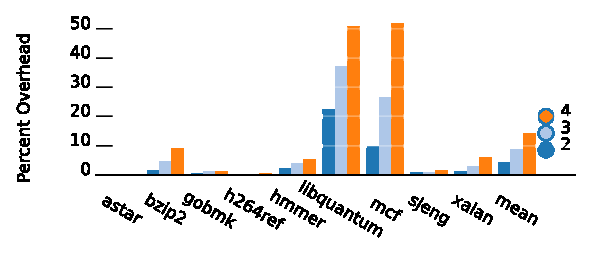
\includegraphics[width=3.4in]{figs/scalability.eps}
        \caption{Performance overhead for 4 TCs.}
        \label{fig:scalability}
    \end{center}
\end{figure}

While future multi-core systems are likely to have a large number of processing 
cores, we note that many security applications will not require many timing 
compartments to be used concurrently. For example, the BYOD application only 
requires two TCs no matter how many cores exist in the system. Similarly, in a 
high-assurance cloud computing environment, the cloud provider can limit the
number of high-assurance virtual machines that can be located on each physical
system while increasing the system utilization by co-locating non-secure
virtual machines with high-assurance ones.

\subsection{Cache Coherence Performance Overhead}

Adding the timing channel protection for snooping coherence bus can introduce 
performance overhead. We evaluate the overhead using Splash2~\cite{splash2} benchmarks on 
gem5. The system we model is the one shown in Figure~\ref{fig:coherent_system}.
We use the same Splash2 benchmarks for Attacker0 and Attacker1, each consists 
of two threads. We terminate the simulation
when thread on core 0 reaches 100M instructions.  Our baseline is a system 
where every other timing channel protection scheme we proposed is implemented 
except for the snooping bus.
We then compare it with the system where the snooping bus is also protected. 
This comparison enables us to quantify the overhead introduced by adding 
cache coherence protection. 

The results are shown in Figure~\ref{fig:splash2}. As can be seen, the overhead 
of adding cache coherence protection is
quite low, with the highest overhead less than 1.5\%. 
%In some cases the 
%protection scheme even outperform the baseline, mainly because the round-robin 
%scheduling may have avoided some snooping bus contention in the baseline 
%scheduling.  
The main reason for the low overhead is that the coherence protocol traffic 
is quite rare in programs, hence the TDM on the
snooping bus does not cause much overhead to the overall program execution 
time.

\begin{figure}
    \begin{center}
        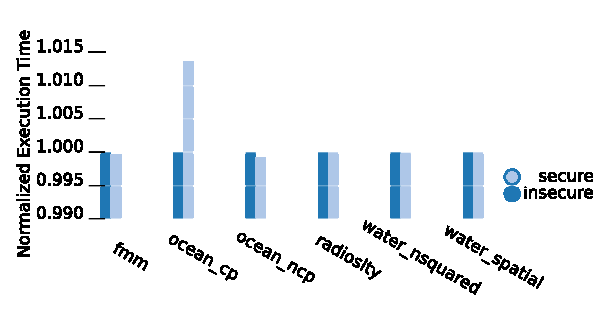
\includegraphics[width=3.4in]{figs/SPLASH.eps}
        \caption{Performance overhead of cache coherence protection.}
        \label{fig:splash2}
    \end{center}
\end{figure}
